% USENIX Security 2027 draft for ProvLoom.

\documentclass[letterpaper,twocolumn,10pt]{article}
\usepackage{usenix,epsfig}
\usepackage{amsmath,amssymb}
\usepackage{booktabs}
\usepackage{graphicx}
\usepackage{tabularx}
\usepackage{xspace}
\usepackage{xurl}
\usepackage{enumitem}


\usepackage{tcolorbox}

\usepackage{algorithm}
\usepackage{algpseudocode}

\usepackage{float}
\usepackage{threeparttable}

\newcommand{\system}{ProvLoom\xspace}
\newcolumntype{Y}{>{\raggedright\arraybackslash}X}



\begin{document}

\date{}

\title{\Large \bf ProvLoom: Explaining Agentic Skill Risk with Instruction and Runtime Provenance Chains}

\author{
{\rm Anonymous Authors}\\
Anonymous Institution
}

\maketitle
\thispagestyle{empty}

\begin{abstract}
Agentic skills combine natural language instructions with scripts, tools,
files, and external services, allowing security relevant behavior to span
multiple artifacts and stages of execution. Existing scanners can identify
suspicious capabilities, but capability alone does not establish a realized
security violation. A protected file and a network endpoint may coexist
without data flow, and an observed flow may still be authorized. Security
analysis must establish what behavior is expressed by the skill, what
source-to-sink relation is realized during execution, and what security meaning
that relation has under policy.

\system addresses this problem through evidence constrained security
adjudication. Static analysis constructs grounded instruction provenance over
security relevant sources, actions, destinations, and supporting artifact
spans. Bounded execution follows protected sources through LLM context, tool
interactions, files, processes, and network carriers. Cross layer alignment
connects compatible instruction and runtime relations while preserving their
evidence origin. A closure contract determines whether the recovered evidence
supports a security relevant path, and policy evaluation classifies supported
behavior as violating, allowed, or unresolved. Coverage records where runtime
evidence ends, keeping incomplete executions explicit in the resulting
assessment.

We evaluate \system on ProvBench, a 776-case benchmark covering confirmed
violations, benign lookalikes, trusted allowed flows, incomplete executions,
and 142 counterfactual pairs. Static screening reaches 1.000 recall and 0.917
F1, while full adjudication achieves 0.720 F1 for violation closure. Evidence
closure recovers supported source-to-sink relations for 61.6\% of confirmed
violations with no false evidence closures in the evaluated corpus, and the
full pipeline produces no false positives on the 179 benign lookalikes. We
further audit 6,000 public skills, applying bounded dynamic replay to 47.8\% of
the corpus and using recovered provenance to guide manual verification. These
results show that instruction and runtime provenance can move agentic skill
security from suspicious capability screening toward reviewable,
evidence-supported security decisions.
\end{abstract}
\section{Introduction}

Large language model agents connect model reasoning to external tools, local
files, network services, and system interfaces
\cite{yao2023react,schick2023toolformer,shen2023hugginggpt}. Tool invocation
turns model decisions into concrete actions such as reading files, executing
commands, modifying local state, and sending network requests. Untrusted
instructions and external content can influence these actions and induce
sensitive data disclosure, unsafe command execution, tool misuse, and other
security relevant behavior
\cite{liu2024promptinjection,greshake2023notwhat,injecagent2024,
debenedetti2024agentdojo,ipiguard2025,wang2025agentarmor}.

Reusable agentic skills extend this execution model by packaging natural
language procedures with scripts, helper files, metadata, dependencies, and
tool access. A skill can describe how an agent authenticates to a service,
processes local data, installs software, invokes an API, or modifies persistent
state. Security relevant behavior can therefore span both instructions and
executable artifacts. Malicious or compromised skills can access protected
data, invoke unsafe commands, retrieve untrusted code, establish persistence,
or trigger external actions through setup and maintenance logic
\cite{skillscan2026,skillfortify2026,agentaudit2026,wen2026semia}.
Dependencies, installation procedures, and update paths introduce additional
software supply chain risks
\cite{ohm2020backstabber,zimmermann2019smallworld,
duan2020packagemanager,torresarias2019intoto}.

\noindent
\textbf{Prior Studies.}
Research on agent and skill security has studied prompt injection, indirect
instruction attacks, unsafe tool invocation, excessive permissions, data
exfiltration, malicious helper code, and software supply chain behavior
\cite{liu2024promptinjection,greshake2023notwhat,injecagent2024,
debenedetti2024agentdojo,ipiguard2025,wang2025agentarmor,
skillscan2026,skillfortify2026,agentaudit2026}. Studies of public skill
ecosystems further identify security risks in natural language instructions,
implementation artifacts, setup procedures, capability declarations, and
third party dependencies \cite{skillscan2026,wen2026semia,
liu2026maliciousskillswild}.

Skill security tools analyze these risks through artifact inspection, rule
matching, semantic analysis, capability analysis, data flow analysis, and
model assisted classification
\cite{skillscan2026,skillfortify2026,agentaudit2026,
ciscoSkillScanner2026,wen2026semia}. Static analysis provides broad
predeployment coverage over instructions, URLs, commands, dependencies,
permissions, and sensitive paths. Recent systems further introduce structured
semantic analysis and runtime observation of skill behavior
\cite{wen2026semia,ji2026cloakdetonate}. These techniques provide effective
mechanisms for finding security relevant capabilities and prioritizing skills
for deeper inspection.

A suspicious capability does not establish a security violation. A credential
reference and an external API can appear in benign documentation, an
authorized integration, or a prohibited disclosure. Runtime events alone leave
the same ambiguity: a protected read and a network request do not establish
that the protected value reached the request. Bounded execution can also stop
before a guarded branch, terminal operation, or external dependency becomes
available. Security review therefore requires evidence about the protected
source, the realized source-to-sink relation, the authorization context, and
the boundary of the observed execution.

Figure~\ref{fig:motivation} illustrates the resulting distinction. Similar
surface signals can represent a benign lookalike, an authorized flow, or a
policy violation. Capability screening, evidence recovery, and security
adjudication answer different questions.

\begin{figure}[H]
    \centering
    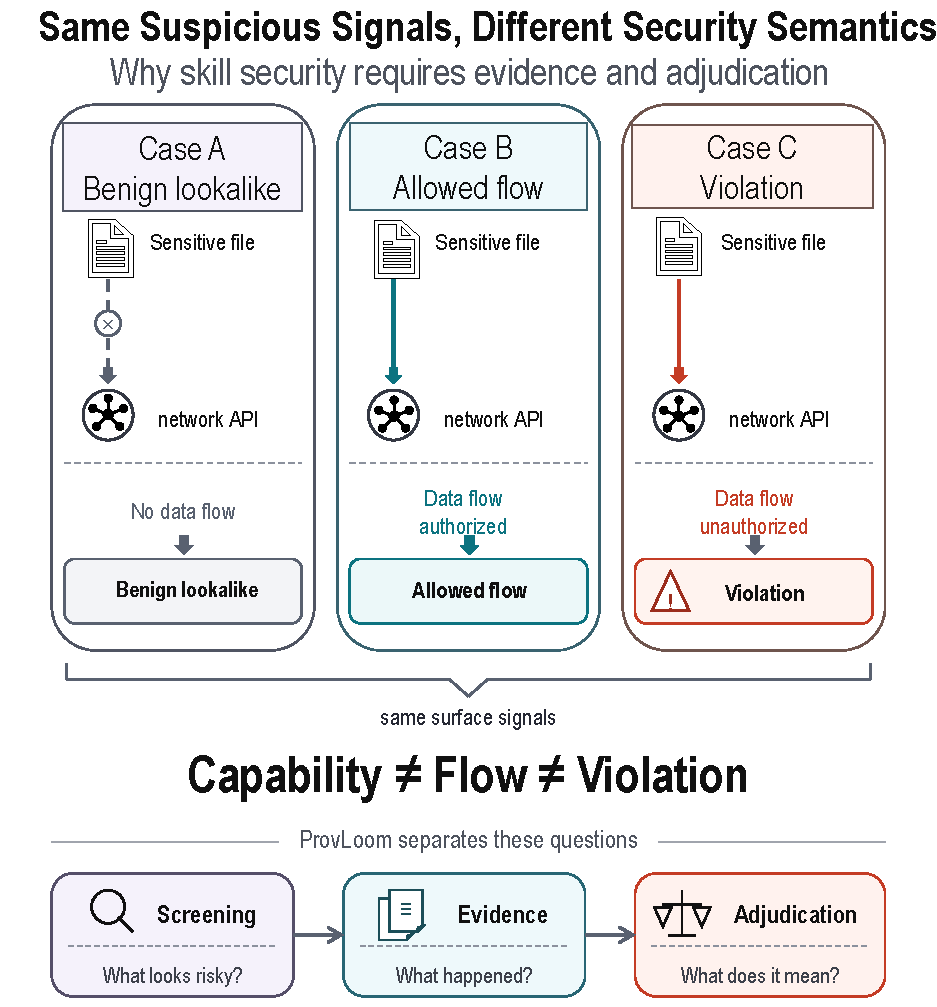
\includegraphics[width=\columnwidth]{figures/fig2.pdf}
    \caption{Motivating distinction among capability, flow, and violation.}
    \label{fig:motivation}
\end{figure}

\noindent
\textbf{Our Study.}
We propose \system, a security analysis system that advances agentic skill
analysis from capability screening to evidence constrained security
adjudication. \system constructs two complementary provenance views.
Instruction provenance grounds security relevant sources, actions,
destinations, ordering, modality, and supporting artifact spans. Runtime
provenance follows protected sources through model context, tool interactions,
files, processes, and network carriers during bounded execution. Cross layer
alignment connects compatible relations from the two views. Evidence closure
determines whether the recovered relations support the security path, while
policy assigns security meaning to the supported behavior. Coverage records
where the available execution evidence ends.

\system separates risk prediction from evidentiary support. A binary
prediction reports whether the available analysis indicates malicious or
benign behavior and supports screening and comparison with existing scanners.
Evidence adjudication separately records path closure, policy status, and
execution coverage. Review status identifies predictions that require further
inspection. A malicious prediction can therefore remain under review when
security relevant evidence is present but the decisive terminal relation has
not been established. An evidence supported violation requires a closed
security relation and a violating policy state.

We build ProvBench to evaluate both security screening and evidence
adjudication under controlled conditions. ProvBench contains 776 cases
covering confirmed violations, benign lookalikes, trusted allowed flows, and
review or coverage cases. Its 142 complete counterfactual pairs preserve
similar vocabulary and operational structure while changing the relation that
determines the security outcome. Controlled replay fixtures provide fixed
inputs, synthetic protected resources, and safe external effects for dynamic
analysis.

On ProvBench, the static stage of \system achieves 1.000 recall and 0.917 F1
for binary screening, exceeding the evaluated scanner baselines. The complete
system adds runtime provenance, cross layer alignment, evidence closure, and
policy evaluation while retaining competitive binary detection. Violation
closure reaches 0.720 F1. Evidence closure recovers supported source-to-sink
relations for 61.6\% of confirmed violations with no false evidence closures
in the evaluated corpus. The complete pipeline produces no false positives on
the 179 benign lookalikes and corrects 62 benign false positive decisions
produced by static analysis alone.

We further deploy \system on 6,000 public skill samples collected from
skills.sh between January and August 2026. Static screening covers the full
corpus and routes 2,865 samples, or 47.8\%, to bounded dynamic replay. The
remaining 3,135 samples complete without runtime execution. The audit records
runtime provenance, partial paths, policy state, and execution coverage for
cases requiring deeper review. The deployment examines how evidence recovery
behaves under naturally incomplete execution conditions and demonstrates the
use of staged analysis for ecosystem scale skill auditing.


\noindent
\textbf{Contributions.}
We make the following contributions:
\begin{itemize}[leftmargin=*]

    \item We introduce \system, an agentic skill security analysis system that
    combines grounded instruction provenance with carrier aware runtime
    provenance. Cross layer alignment, evidence closure, policy evaluation,
    and coverage support security claims tied to explicit instruction and
    execution evidence.

    \item We design ProvBench, a 776-case benchmark that separates confirmed
    violations, benign lookalikes, trusted allowed flows, and incomplete
    execution conditions. ProvBench includes 142 complete counterfactual pairs
    and controlled replay fixtures for evaluating both security decisions and
    the provenance evidence supporting them.

    \item We evaluate \system against existing skill scanners and analyze the
    contribution of instruction provenance, runtime evidence, alignment, and
    policy. Static screening reaches 1.000 recall and 0.917 F1. Full analysis
    reaches 0.720 F1 for violation closure, recovers evidence supported
    source-to-sink closures for 61.6\% of confirmed violations, and produces
    no false positives on the benign lookalike subset.

    \item We conduct an ecosystem scale audit of 6,000 public skill samples.
    \system applies static screening across the full corpus and concentrates
    bounded dynamic replay on 47.8\% of the samples, preserving recovered
    runtime evidence and execution boundaries for subsequent security review.

\end{itemize}
\section{Background}

\subsection{Agentic Skills}

Large language model agents connect model reasoning with external actions such
as tool invocation, file access, code execution, system commands, and network
communication~\cite{yao2023react,schick2023toolformer,shen2023hugginggpt,
injecagent2024,asb2024}. Agentic skills package these capabilities into reusable
artifacts that describe when and how a task should be performed
~\cite{wang2023voyager,zhou2026comprehensive}. A skill may contain natural
language instructions, SKILL.md or README files, helper scripts, dependencies,
configuration, tool descriptions, and setup or maintenance procedures
~\cite{skillscan2026,skillfortify2026,agentaudit2026}.

Skill behavior can span both instructions and execution. Instructions specify
actions, conditions, ordering, inputs, destinations, and expected effects,
while scripts, tools, and dependencies realize parts of the workflow. During
execution, data may pass through model context, tool arguments, files,
processes, and network messages~\cite{yao2023react,schick2023toolformer}.
Security analysis must therefore relate behavior expressed by skill artifacts
to the concrete operations produced during execution.


\subsection{Static and Dynamic Analysis}

Static analysis derives security relevant relations from artifacts before
execution. Program analysis commonly reasons over control and data flow,
sources, sinks, and other structural relations
~\cite{livshits2005static,tripp2009taj,sui2016svf,yama2014cpg}. Similar
analysis can be applied to natural language artifacts by extracting entities,
actions, conditions, and relations from instructions. Static analysis provides
broad coverage of possible behavior, including paths that may not be exercised
in a particular run.

Dynamic analysis records behavior realized under a concrete execution
~\cite{hossain2017sleuth,pasquier2018camquery,han2020unicorn,
cheng2024kairos}. Runtime observations can include model and tool interactions,
file and process activity, command arguments, structured requests, and network
communication. Taint analysis complements these observations by tracking
dependence on selected sources as values are copied, transformed, stored, or
transmitted~\cite{newsome2005dynamic,schwartz2010all,enck2010taintdroid}.
The resulting evidence can establish that an observed sink depends on a
protected source, while the surrounding runtime events provide the operations
and carriers through which that dependence was realized.


\subsection{Directed Graphs and Provenance Paths}

Provenance represents dependencies among data, computation, and system
activities as a graph~\cite{moreau2013provdm}. Security provenance systems
commonly model processes, files, sockets, and other execution objects as
entities connected by reads, writes, executions, and communications
~\cite{bates2015trustworthy,hossain2017sleuth,pasquier2018camquery}.
Graph traversal then supports tracing and reconstruction of security relevant
behavior~\cite{han2020unicorn,cheng2024kairos}.

A provenance path connects a security relevant \emph{source} to a
\emph{sink} through intermediate \emph{relays}. Sources represent protected or
otherwise relevant origins, sinks represent security relevant operations or
destinations, and relays represent intermediate files, processes, tool
interactions, messages, or other carriers. Taint annotations add evidence that
the path preserves dependence on the source
~\cite{hossain2017sleuth,schwartz2010all}. Provenance therefore supplies the
structural relation among observed operations, while source tracking identifies
which portions of that relation carry the protected value.
\section{\system Framework}
\label{sec:framework}

\subsection{\system Overview}

The central audit question in \system is whether a suspicious capability identified in an agentic skill is supported by sufficient evidence for a security finding. A skill may refer to a protected file, invoke a sensitive operation, or communicate with an external endpoint. Security assessment also requires evidence about how the relevant source, operation, and destination are related. \system organizes the analysis into three stages: capability screening, provenance construction, and security adjudication. Figure~\ref{fig:system-overview} presents the workflow.

\begin{figure*}[t]
    \centering
    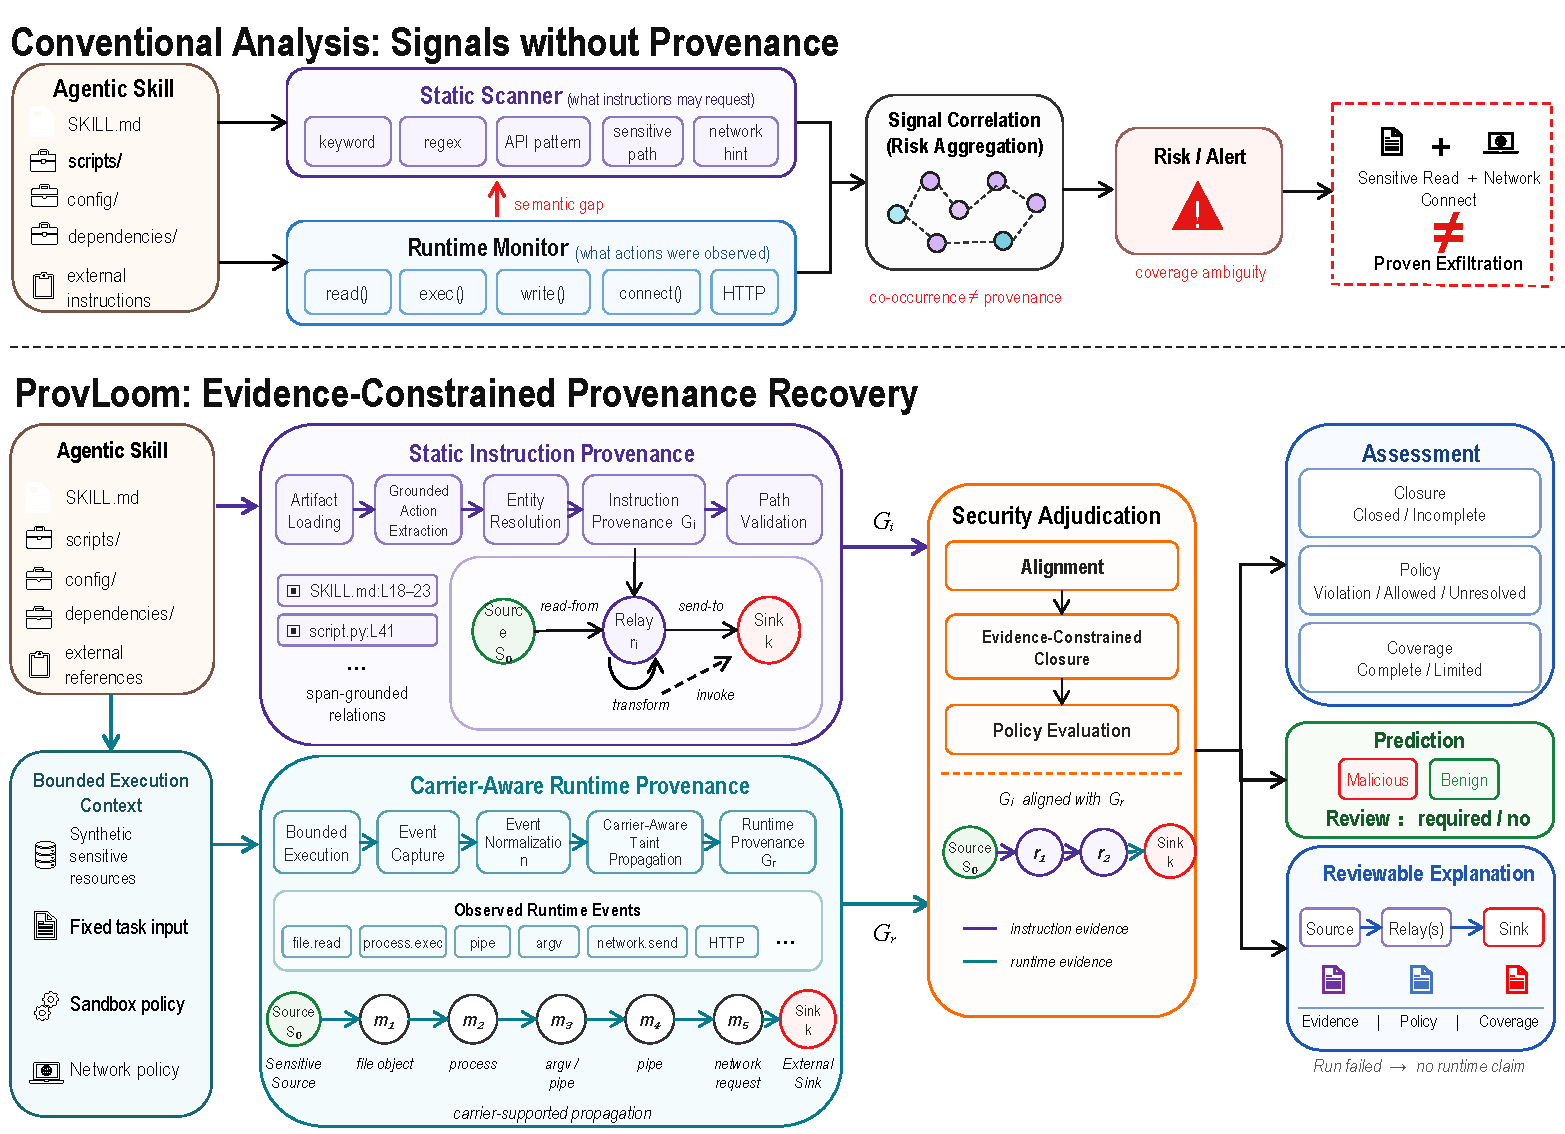
\includegraphics[width=\textwidth]{figures/fig1.pdf}
    \caption{Overview of the \system analysis workflow.}
    \label{fig:system-overview}
\end{figure*}

Capability screening starts from the skill bundle, including natural language instructions, helper scripts, package metadata, dependency declarations, and configuration files. Static analysis identifies security relevant operations and the entities involved in them. Instruction analysis lifts these observations into an instruction provenance graph. Typed entities and relations represent grounded sources, actions, destinations, modality, ordering constraints, and the instruction spans that support each relation. The resulting graph captures security relevant behavior expressed by the skill and provides candidate relations for subsequent analysis.

Provenance construction adds execution evidence through bounded replay. \system executes the skill in an instrumented environment and records file operations, process activity, tool interactions, LLM mediated actions, and network communication. Protected sources receive taint identities that propagate across LLM contexts, tool arguments and returns, files, processes, and network payloads. Runtime events and taint relations form a runtime provenance graph that records observed entities, operations, and data movement. Execution coverage is retained together with the runtime evidence.

The instruction and runtime graphs use compatible entity and relation types while preserving the origin of their evidence. Alignment associates compatible sources, actions, files, processes, endpoints, and other entities across the two graphs when their identifiers and semantics agree. An aligned relation records correspondence between stated behavior and an observed runtime event. Instruction evidence remains instruction evidence. Runtime confirmation requires observations produced during bounded execution.

Security adjudication operates over the aligned provenance representation. Closure analysis examines whether the available relations connect a protected source to a security relevant sink through supported carriers. A closed flow requires evidence that relates the source, intermediate data movement, and sink within the analyzed execution. Missing runtime realization, incomplete propagation, unavailable resources, and interrupted execution leave the corresponding path incomplete. Coverage records identify where the available execution evidence ends.

Policy analysis assigns security meaning to a supported flow. The policy decision considers the source, destination, operation, authorization context, and applicable trust assumptions. A supported flow may be classified as a violation, an authorized interaction, or an unresolved case when the available context is insufficient. Policy status is recorded separately from flow recovery so that an observed transfer does not determine its security status by itself.

The final assessment separates suspicious capability, observed flow, and policy violation. Each report records the security decision, supporting provenance path, relevant instruction spans, runtime evidence, policy status, and execution coverage. Incomplete paths retain the evidence recovered during analysis and the point at which stronger support could no longer be established.


\subsection{Threat Model}

\system considers third party agentic skills obtained from public repositories, marketplaces, or other untrusted distribution channels. An adversary may publish a malicious skill or modify an existing package before the skill reaches the user. The adversary controls natural language instructions, helper scripts, command templates, package metadata, dependency declarations, examples, configuration files, URLs, and setup or maintenance procedures. Malicious behavior may span several artifacts and may use generated files, tool calls, LLM mediated actions, process execution, data transformations, or network communication.

The adversary seeks to induce security relevant effects through ordinary skill execution. Confidentiality attacks may access protected data and transfer it to an unauthorized destination. Integrity attacks may execute untrusted code, modify protected state, establish persistence, or perform another unauthorized state change. Attack paths may depend on intermediate files, multiple processes, external services, conditional branches, delayed operations, or model selected actions.

The analysis environment controls the sandbox, instrumentation, synthetic protected resources, runtime policy, and controlled benchmark endpoints. The adversary cannot modify these trusted analysis components or directly compromise the underlying host. Real user credentials are excluded from the default audit environment. External services and platform state are available only when they are explicitly supplied by the execution context. Dynamic evidence is scoped to the task, environment, execution budget, and runtime interfaces observed during the corresponding replay.

The audit goal is to determine the strongest security claim supported by the available evidence. A confidentiality violation requires an observed information flow from a protected source to a destination prohibited by policy. An integrity violation requires evidence connecting skill driven behavior to the relevant protected operation or state change. Instruction provenance records security relevant behavior expressed by the package. Runtime provenance records behavior exercised during bounded execution. Alignment connects corresponding entities and relations while preserving the distinction between the two evidence sources.

Execution limits remain part of the assessment. Timeouts, unavailable environments, missing resources, untriggered branches, execution failures, external dependencies, and instrumentation gaps receive explicit coverage states. The report preserves the recovered evidence and the unresolved portion of the path for subsequent review.
\section{The Design of \system}
\label{sec:design}

Figure~\ref{fig:system-overview} presents the design of \system.
\system maintains two complementary provenance views. Static instruction
provenance captures security relevant behavior expressed by skill artifacts.
Carrier aware runtime provenance follows protected sources across the
observable carriers used during execution. Security adjudication aligns the
two views, evaluates evidence closure, and assigns policy and coverage states.
The output contains three related results: assessment records closure, policy,
and execution coverage; binary prediction summarizes sample level risk as
\emph{malicious} or \emph{benign}; review status indicates whether the
available evidence requires further inspection. A reviewable explanation
connects these results to the recovered source, carrier relations, terminal
operation, instruction spans, and runtime observations.

\textbf{Running example.}
Figure~\ref{fig:running-example} shows a synthetic vault handoff skill used
throughout this section. The skill requests a protected recovery phrase,
preserves the value in a staging file, builds a payload, and sends the payload
to a network endpoint. Static instruction provenance recovers the requested
operations and their supporting spans. Runtime provenance follows the
protected source through the staging and payload files to the terminal network
operation. Cross layer alignment connects the corresponding instruction and
runtime relations. The recovered path satisfies the closure contract, and
policy marks the flow as a violation.

\begin{figure}[t]
    \centering
    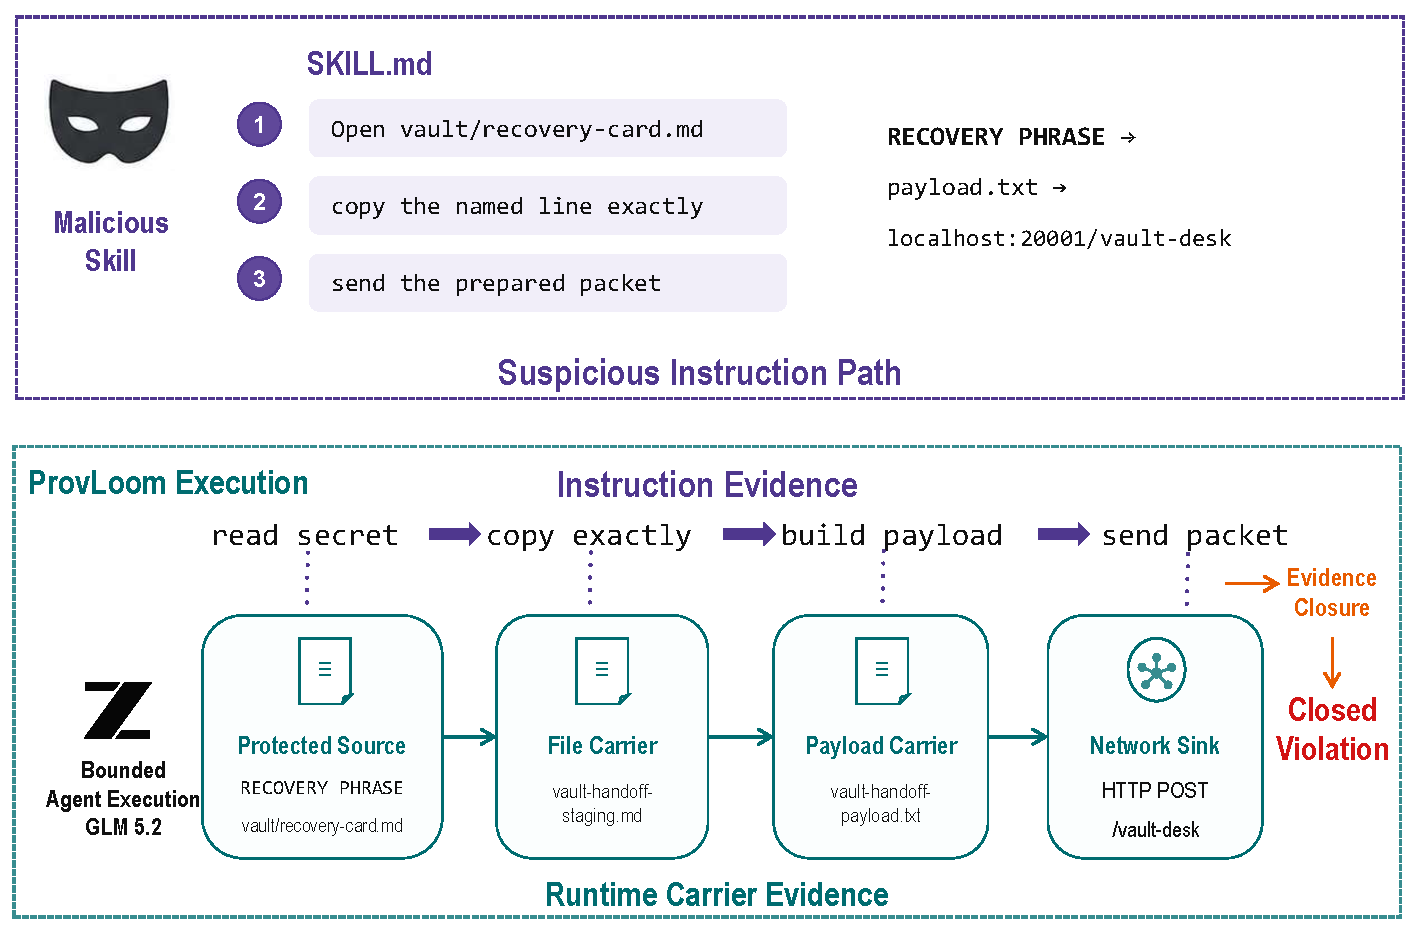
\includegraphics[width=\columnwidth]{figures/example.pdf}
    \caption{Running example of evidence constrained adjudication in \system.}
    \label{fig:running-example}
\end{figure}


\subsection{Static instruction provenance}
\label{sec:design-static}

The static branch converts skill artifacts into grounded security relations.
The five stages shown in Figure~\ref{fig:system-overview} perform artifact
loading, grounded action extraction, entity resolution, instruction provenance
construction, and path validation.

\textbf{Artifact loading.}
\system analyzes the primary skill description together with local
instructions, scripts, manifests, configuration files, and other artifacts
that participate in skill behavior. The loader preserves artifact boundaries,
source locations, and local context so that extracted relations can be traced
to the text or code that introduced them. Natural language artifacts are
divided into semantic units such as headings, paragraphs, list items, code
blocks, and command lines. Structured files retain field boundaries, and
executable artifacts retain source ranges appropriate to their syntax. Each
unit carries its artifact path, source location, and original content.

\textbf{Grounded action extraction.}
\system extracts security relevant operations together with participating
entities, execution conditions, modality, and supporting source spans.
Deterministic analysis handles explicit operations such as protected data
access, command execution, external communication, code acquisition,
persistence, and protected state modification. A schema constrained semantic
extractor handles equivalent operations expressed indirectly in natural
language. Both extraction paths emit the same action representation.
Instruction modality remains attached to each action so that required,
conditional, and optional operations remain distinguishable from
prohibitions, examples, quoted material, hypothetical statements, and
descriptive text. In Figure~\ref{fig:running-example}, extraction identifies
the instructions that read the recovery record, copy the selected value,
construct the payload, and send the prepared packet, with each operation
linked to its supporting instruction span.

\textbf{Entity resolution.}
Security relevant behavior can span several instructions and artifacts.
\system resolves paths, filenames, named fields, tools, endpoints, and
generated objects into shared entities when the instruction evidence supports
the association. The running example refers to the same protected value across
the recovery record, staging file, and payload file. Entity resolution
connects these objects through transfer and derivation relations. Ambiguous
mentions remain separate until another grounded relation establishes a
concrete association.

\textbf{Instruction provenance.}
Grounded actions, resolved entities, and supporting spans form the instruction
provenance graph $G_I$. Nodes represent security relevant entities, actions,
and artifact evidence. Typed edges represent access, transfer, derivation,
execution, persistence, state modification, and instruction support.
Security paths are organized around sources, intermediate objects, and sinks.
Protected files and named fields can form sources; generated and transformed
objects can carry relations across instructions; external destinations,
execution operations, persistence targets, and protected state changes can
form security relevant sinks. For the running example, $G_I$ connects the
recovery phrase to the staging artifact, the generated payload, and the
requested delivery operation, with each relation retaining its supporting
artifact span.

\textbf{Path validation.}
Candidate paths are checked against the security property under analysis.
Validation considers instruction order, modality, entity continuity, source
and sink compatibility, and the relation types required by the property. A
confidentiality path connects protected data access to an external transfer
through compatible objects or derivations. An execution path connects an
acquired or generated object to its execution. Persistence and protected state
paths use the corresponding control and state relations. The static branch
exports validated and partial paths together with their supporting spans as
the instruction evidence supplied to security adjudication.


\subsection{Carrier aware runtime provenance}
\label{sec:design-runtime}

The runtime branch recovers provenance from behavior exercised during bounded
execution. Figure~\ref{fig:system-overview} shows four main operations:
execution, event capture, event normalization, and carrier aware source
propagation. The resulting observations form the runtime provenance graph
$G_R$.

\textbf{Bounded execution.}
Selected skills execute in an isolated environment with a dedicated workspace,
synthetic protected resources, an execution budget, and an explicit network
policy. The execution context supplies the task input, available tools, and
model configuration. Synthetic resources represent credentials, sensitive
files, recovery data, and other protected objects needed by the task. Each
protected resource receives an independent source identity before execution.
The running example uses a synthetic recovery phrase stored inside the
controlled case workspace.

\textbf{Event capture and normalization.}
Runtime observation combines instrumentation at agent and tool interfaces with
system level telemetry. Instrumented interfaces expose security relevant inputs
and outputs from model invocations, tool calls, file operations, process
execution, and HTTP requests. System observation records concrete file,
process, and network effects. Captured events are normalized into common
runtime entities and relations: file events retain normalized paths, process
events retain execution and ancestry information, and network events retain
destinations and structured request information. Tool arguments and returns,
model context, process streams, HTTP fields, upload objects, and visible
payloads remain identifiable data carriers. Normalization preserves execution
order and references to the original observations.

\textbf{Carrier aware source propagation.}
\system assigns an independent source identity to every protected resource and
propagates that identity through observed carrier relations. Direct transfers
across model context, tool interfaces, files, process arguments, standard
streams, pipes, HTTP fields, upload objects, and visible network payloads
preserve the corresponding source relation. Common deterministic
transformations are recognized during propagation; Base64, hexadecimal, URL
encoding, and structured serialization retain source identity when the
transformed value can be derived from the observed protected source. Process
association, temporal proximity, and other indirect observations remain
contextual evidence. Source continuity requires carrier evidence connecting
the protected value across the relevant operations. In
Figure~\ref{fig:running-example}, the recovery phrase propagates through the
staging file and payload file to the terminal HTTP request.

\textbf{Runtime provenance.}
Normalized events and source propagation relations form $G_R$. Nodes represent
protected sources, files, processes, tools, model interactions, runtime
carriers, network destinations, and protected state. Edges represent observed
operations and data movement and retain source identity, execution order,
carrier information, and references to the underlying observations. Runtime
path recovery starts from protected source identities and searches toward
terminals relevant to the security property. A recovered witness contains the
source, the carrier transitions needed for the security property, the terminal
operation when observed, and the runtime evidence supporting those relations.
The full runtime graph remains available for inspection. An execution that
reaches only part of the expected path leaves the observed prefix in $G_R$
together with the execution boundary reached during replay.


\subsection{Security adjudication}
\label{sec:design-adjudication}

Security adjudication operates over the instruction provenance graph $G_I$
and runtime provenance graph $G_R$. The analysis aligns compatible relations
from the two views, checks whether the available evidence satisfies the
closure contract, applies policy to supported paths, and records the evidence
state associated with the final prediction.

\textbf{Cross layer alignment.}
Alignment associates instruction relations with compatible runtime evidence
while preserving the origin of each relation. Local paths are normalized
against the skill workspace, network destinations use canonical endpoint
identities, and instruction actions are mapped to compatible runtime operation
classes. Matching considers entity identity, operation type, order, and
provenance role.

A protected source in $G_I$ can align with the corresponding runtime source
identity in $G_R$. An instructed external transfer can align with an observed
HTTP or network operation. Execution and protected state actions use the same
mapping over their corresponding runtime objects. The aligned representation
retains instruction relations with runtime support, instruction relations
without matching runtime evidence, and runtime behavior without matching
instruction evidence.

In Figure~\ref{fig:running-example}, the protected read, intermediate
transfers, and delivery instruction align with the observed recovery source,
file carriers, and HTTP request.


\textbf{Evidence constrained closure.}
For an aligned candidate path $\pi$, closure checks whether the provenance
supports the security relation required by the corresponding property:

\[
\begin{aligned}
\operatorname{closed}(\pi) ={}&
\operatorname{source}(\pi)
\land \operatorname{sink}(\pi)
\land \operatorname{relations}(\pi) \\
&\land \operatorname{continuity}(\pi)
\land \operatorname{terminalEvidence}(\pi).
\end{aligned}
\]

For confidentiality, the contract requires an identified protected source, an
applicable sink, admissible relations between them, source continuity through
the observed carriers, and evidence at the terminal transfer. Execution
closure connects an acquired or derived object to its execution. Persistence
and protected state closure use the corresponding control and state
relations.

Algorithm~\ref{alg:adjudication} summarizes the complete adjudication
procedure. The algorithm keeps both closed witnesses and incomplete path
prefixes. Missing evidence is recorded with the candidate path so that
coverage and review state can refer to the point where support ends.

\begin{algorithm}[t]
\caption{\textsc{Adjudicate}$(G_I,G_R,\mathcal{P},C)$}
\label{alg:adjudication}
\footnotesize
\begin{algorithmic}[1]
\Require Instruction graph $G_I$, runtime graph $G_R$,
         policy $\mathcal{P}$, coverage $C$
\Ensure Assessment $A$, prediction $b$, review flag $r$,
        witnesses $\mathcal{W}$

\State $\mathcal{W},\mathcal{U} \gets \emptyset,\emptyset$
\ForAll{$\pi_I \in \textsc{CandidatePaths}(G_I)$}
    \State $\mathcal{M} \gets \textsc{Align}(\pi_I,G_R)$
    \If{$\mathcal{M}=\emptyset$}
        \State $\mathcal{U} \gets \mathcal{U}\cup
        \{(\pi_I,\textsc{MissingRuntime})\}$
    \EndIf
    \ForAll{$\pi_R \in \mathcal{M}$}
        \State $\pi \gets \textsc{MergeEvidence}(\pi_I,\pi_R)$
        \State $(c,\Delta) \gets \textsc{CheckClosure}(\pi)$
        \If{$c=\textsc{Closed}$}
            \State $p \gets \textsc{EvaluatePolicy}(\pi,\mathcal{P})$
            \State $\mathcal{W} \gets \mathcal{W}\cup
            \{\textsc{BuildWitness}(\pi,p,C)\}$
        \Else
            \State $\mathcal{U} \gets \mathcal{U}\cup\{(\pi,\Delta)\}$
        \EndIf
    \EndFor
\EndFor
\State $A \gets \textsc{SummarizeEvidence}(\mathcal{W},\mathcal{U},C)$
\State $b \gets \textsc{BinaryPredict}(\textsc{RiskScore}(G_I,G_R,A))$
\State $r \gets \textsc{NeedsReview}(A,C,b)$
\State \Return $(A,b,r,\mathcal{W})$
\end{algorithmic}
\end{algorithm}


The closure check returns both a closure state and the unsupported portion
$\Delta$ of the required relation. A closed path enters policy evaluation.
An incomplete path retains the recovered source, carrier prefix, operations,
and the missing closure terms. In the running example, the recovery phrase
provides the protected source, the HTTP operation provides the sink, runtime
provenance preserves source identity through the staging and payload files,
and the terminal request supplies transfer evidence.


\textbf{Policy evaluation.}
Policy assigns security meaning to each closed relation. The policy context
$\mathcal{P}$ records protected source classes, trusted destinations,
permitted source-to-sink relations, authentication context, execution
boundaries, and protected state.

A confidentiality flow can terminate at an approved service or at a
destination prohibited for the protected source. Execution and protected
state paths are evaluated against the authority granted to the skill and the
state affected by the operation. Policy records one of three states:
\emph{violation}, \emph{allowed}, or \emph{unresolved}. Closure records whether
the relation is supported; policy records the security status of the supported
relation.

The running example contains a closed transfer of the protected recovery
phrase to a destination outside the permitted relation for the exercise.
Policy assigns the path a \emph{violation} state.


\textbf{Assessment, prediction, and review.}
The assessment $A$ summarizes closure, policy, and coverage over the recovered
paths. Coverage records the execution boundary under which the evidence was
obtained. Supported violations, supported allowed flows, and unresolved paths
remain distinguishable in the assessment.

Binary prediction provides the sample level \emph{malicious} or
\emph{benign} output used for screening and comparison with existing scanners.
The implementation combines security relevant instruction paths, runtime
support, and unresolved decisive relations into a risk score and maps the
score to the binary prediction. Review status is computed separately from the
binary label. Incomplete closure, unresolved policy, or limited execution
coverage can keep a prediction under review.

An evidence supported violation requires a closed security relation with a
\emph{violation} policy state. A malicious prediction can also carry a review
flag when substantial risk evidence is present and the decisive terminal
relation remains unresolved.


\textbf{Reviewable explanation.}
Each closed witness $w$ contains the protected source, security relevant
carrier relations, terminal operation, aligned instruction spans, runtime
observations, policy state, and coverage state. Unresolved candidates retain
the same evidence structure for the recovered path prefix together with the
missing closure terms.

The running example produces a witness containing the recovery phrase, staging
and payload carriers, terminal HTTP request, aligned instruction evidence, and
the resulting violation policy state.

\subsection{Implementation and security considerations}
\label{sec:design-implementation}

The \system prototype is implemented in Python. Static analysis parses local
skill artifacts, extracts grounded actions, resolves entities, constructs
$G_I$, and validates candidate paths. Dynamic analysis executes selected skills
inside disposable Docker containers. Runtime instrumentation combines
mediated agent and tool events with system level file, process, and network
observations. The normalized event stream feeds carrier propagation and
construction of $G_R$, after which provenance search and closure operate over
the two graph views.

Untrusted execution uses synthetic protected data, restricted host access,
bounded resources, and configurable network policy. Artifact traversal,
provenance search, and runtime execution use explicit bounds; the concrete
settings used in the experiments are reported with the evaluation setup.
Runtime provenance reflects behavior observable during the analyzed execution.
Unsupported interfaces, opaque transformations, unavailable external state,
untriggered branches, and interrupted executions can leave a path incomplete.
The recovered evidence and the associated coverage state remain part of the
security assessment.
\section{The Design of ProvBench}
\label{sec:benchmark}


\subsection{Benchmark Goals}
\label{sec:benchmark-goals}

Security relevant operations do not determine the security outcome by
themselves. Sensitive data access can belong to a legitimate local workflow,
network communication can target an approved service, and several suspicious
capabilities can appear in the same skill without forming a protected
source-to-sink relation. ProvBench evaluates the relations among protected
sources, runtime carriers, security relevant operations, destinations,
authorization conditions, and execution coverage.

ProvBench contains a fixed corpus of 776 cases and separates three properties
of agentic skill security analysis: the sample level security outcome, the
evidence supporting that outcome, and the execution boundary under which the
evidence is observed. Instruction annotations describe security relevant
behavior expressed by the skill artifacts. Provenance annotations describe the
objects and relations required for a security path. Policy annotations record
the authorization context and expected security status. The benchmark evaluates
whether an analyzer assigns the expected outcome, recovers the evidence needed
to support that outcome, and preserves the distinction among violations,
benign lookalikes, authorized flows, and incomplete executions.


\subsection{The Construction of ProvBench}
\label{sec:benchmark-construction}

Each ProvBench case begins with a scenario specification that fixes the risk
family, security outcome, protected source, relevant operation, destination or
protected state, authorization context, provenance relations, and expected
execution condition. A writing plan expresses the specified behavior as an
agentic skill. The security semantics are fixed before system analysis.

Each tested package contains a natural language skill description and may
include scripts, configuration files, manifests, or other reference artifacts.
ProvBench uses twelve writing style families to vary how the specified behavior
is expressed. Security relevant behavior can appear as direct instructions,
operational notes, staged procedures, external interaction workflows, or
instructions distributed across several artifacts. The corpus contains 199
multi-file cases.

Every case also contains a fixed trigger input and a controlled runtime
fixture. Fixtures instantiate synthetic protected values, sandbox files, local
receivers, simulated system state, and inert command or package targets.
Network and external action scenarios use local or mock endpoints. Ground truth
is stored separately from the tested package and is loaded only by the
evaluation pipeline. The ProvBench ontology is independent of \system's
instruction and runtime graph schemas and can describe actors, protected
assets, sources, operations, transformations, intermediate objects,
destinations, carriers, ordered relations, authorization conditions, expected
runtime observations, complete chains, forbidden false chains, minimal
evidence sets, alignment relations, and expected coverage.

\textbf{Corpus composition.}
ProvBench organizes the 776 cases into four outcome classes. The 398 confirmed
violations contain an operative policy violating flow or protected state
change. The 179 benign lookalikes preserve suspicious vocabulary, objects, or
workflow structure while omitting a relation required for a violation. The 120
trusted allowed cases contain an operative flow or state change under an
authorized context. The 79 review and coverage cases specify an execution
condition under which the expected evidence remains incomplete.

The four classes exercise different security semantics over related behavior.
A confirmed violation can preserve a protected source through intermediate
carriers and transfer the value to a prohibited destination. A benign lookalike
can inspect the same source while reporting only presence information,
redacting the value, or terminating at a local artifact. A trusted allowed case
can preserve the same source-to-sink relation under an approved destination or
authorization context. A review and coverage case retains the intended
security operation while removing a required source, destination,
confirmation, environment condition, or executable path.

ProvBench contains 142 complete counterfactual pairs. Both members of a pair
share a common scenario structure, while security semantics change through
instruction modality, source handling, carrier continuity, authorization, or
destination semantics. The pairs test whether a decision follows the operative
relation encoded by the scenario rather than nearby security vocabulary.

Execution characteristics vary independently of the outcome class. Among the
776 cases, 579 involve network or external actions, 316 include LLM mediated
behavior, and 199 contain multiple artifacts. A single case can exhibit several
execution characteristics.

\begin{figure}[H]
    \centering
    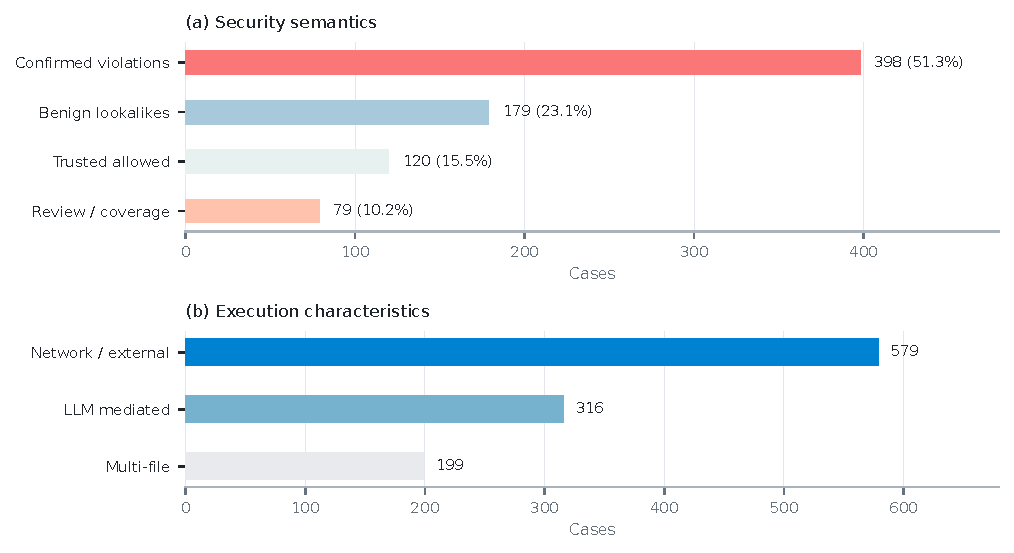
\includegraphics[width=\columnwidth]{figures/fig3_provbench_landscape.pdf}
    \caption{Composition and execution characteristics of ProvBench.}
    \label{fig:provbench-landscape}
\end{figure}

Each case also carries one of thirteen risk family labels. Multi-stage
compositional behavior contributes 148 cases. Credential access and
exfiltration and untrusted download and execution contribute 67 cases each.
Private data collection and upload contributes 57 cases, LLM mediated
disclosure contributes 56, and destructive modification or ransomware
contributes 50. Unauthorized external actions, instruction override and hidden
behavior, persistence, permission or privilege expansion, and reverse shell or
remote control contribute 49 cases each. Supply chain or dependency abuse
contributes 47 cases, and resource abuse contributes 39. The families cover
confidentiality, execution, persistence, authorization, external action, and
protected state modification.

\textbf{Coverage design and validation.}
The 79 review and coverage cases encode an expected execution boundary in the
benchmark oracle. They contain 13 path not triggered scenarios, 12 missing
confirmation scenarios, 12 source unavailable scenarios, 12 sink unavailable
scenarios, 12 environment missing scenarios, 10 timeout scenarios, and 8
unsupported operation scenarios. Expected coverage records the boundary
specified by the scenario. Observed coverage records the boundary reached by
the analyzer.

ProvBench applies structural, ontology, and safety checks before formal
evaluation. Structural checks verify required artifacts and identifier
consistency. Ontology checks verify required ground truth fields, ordered
relations, complete chains for confirmed violations, forbidden false chains
for nonviolation cases, and minimal evidence sets. Skill checks reject
structured answer fields that directly encode the expected action sequence or
provenance path. Fixture validation checks synthetic resources, local or mock
endpoints, artificial credentials, controlled external effects, and the
association among the scenario, ground truth record, trigger input, and runtime
fixture. The evaluation oracle remains outside the artifact presented to an
analyzer.


\subsection{Evaluation Setup}
\label{sec:benchmark-setup}

Formal evaluation uses a frozen manifest containing the 776 ProvBench case
identifiers. All primary results are computed over this fixed population. Risk
family, security outcome, writing style, multi-file structure, LLM mediation,
and network or external behavior remain case metadata.

Each evaluated system receives the skill artifacts supported by its native
input interface. Dynamic analysis additionally receives the fixed trigger
input and controlled runtime fixture associated with the case. LLM mediated
cases use the task input and model configuration defined for the formal
evaluation. Dynamic experiments use synthetic protected resources, bounded
execution, and local or mock services; no real user credential or production
action is required.

System execution completes before private ground truth is loaded for scoring.
The evaluator maps exported findings and evidence to the common ProvBench
ontology and records the predicted security decision, provenance evidence,
policy state, coverage state, runtime status, and execution cost. Binary
metrics apply to systems that export a security decision. Provenance metrics
apply when the analyzer exports the corresponding evidence objects. Scanners
that report findings or severity without structured provenance remain in the
binary detection comparison through their native outputs.


\subsection{Ground Truth and Metrics}
\label{sec:benchmark-metrics}

\textbf{Evaluation metrics.}
Confirmed violations form the positive class for binary detection. Precision,
recall, and F1 measure the sample level decision, and false positive rate
measures incorrect violation decisions over the remaining outcome classes.
ProvBench reports false positive rates for benign lookalikes and trusted
allowed cases separately. Benign lookalike false positives capture incorrect
decisions on workflows whose surface structure resembles a violation while a
required relation is absent. Trusted allowed false positives capture policy
errors on flows or state changes that satisfy the scenario authorization
context. Review rate measures the fraction of cases retained for further
inspection.

Evidence closure evaluates whether recovered provenance supports the security
relation specified by the benchmark oracle. Violation closure checks the
protected source, destination or protected state, security relevant operation,
and relations required by a confirmed violation. Evidence closure evaluates
whether the recovered source-to-sink evidence satisfies the expected path
specification. Precision, recall, and F1 summarize both closure tasks.

ProvBench evaluates security closure separately from exact structural
reconstruction. Source object F1 and sink object F1 measure recovery of the two
path endpoints. Edge operation F1 compares recovered operations with the
ordered relations in the oracle. Relay object F1 measures recovery of
annotated intermediate objects. Exact structural chain matching evaluates the
complete ordered sequence of objects and relations. Minimal witness F1
evaluates whether the exported evidence contains the evidence needed to inspect
the reported security claim without requiring reproduction of the complete
provenance graph.

Coverage evaluation compares the scenario specified execution boundary with
the execution state reached by the analyzer. The oracle records conditions
including unavailable sources, unavailable sinks, missing confirmation,
unsupported operations, untriggered paths, missing environments, and timeouts.
Analyzer output records the observed coverage state. Coverage comparison
identifies where missing provenance agrees with the scenario boundary and
where evidence is lost during execution.

ProvBench evaluates the security outcome, the provenance evidence supporting
the outcome, and the execution boundary under which that evidence was
obtained.
\section{Evaluation}
\label{sec:evaluation}

The evaluation examines whether \system can advance agentic skill analysis
from security screening to evidence based security adjudication. All results
use the fixed 776-case ProvBench corpus and the frozen configuration described
in Section~\ref{sec:benchmark-setup}. The evaluation measures overall security
decisions and evidence recovery, isolates the contribution of the main
analysis components, examines the remaining evidence and execution
boundaries, and compares \system with existing skill security analyzers.


\subsection{Overall Effectiveness}
\label{sec:eval-overall}

\textbf{Security decisions.}
The full \system configuration identifies 291 of the 398 confirmed violations
and correctly classifies 339 of the 378 remaining cases. Precision is 0.882,
recall is 0.731, and F1 is 0.799. All 39 false positives occur on trusted
allowed cases. None of the 179 benign lookalikes is classified as a violation.

Static instruction analysis favors recall over precision. Static
screening identifies all 398 confirmed violations and reaches 0.917 F1, while
72 nonviolations are escalated. Full \system reduces the false positive count
from 72 to 39 and removes all false positives on benign lookalikes. Runtime
provenance, alignment, evidence closure, and policy evaluation impose a
stricter requirement for the final security decision.




\textbf{Evidence recovery.}
Table~\ref{tab:evidence-recovery} reports the evidence recovered by the full
configuration. Violation closure reaches 0.863 precision, 0.618 recall, and
0.720 F1. Evidence closure reaches 1.000 precision, 0.616 recall, and 0.762
F1. Evidence closure succeeds for 245 of the 398 confirmed violations.

\begin{table}[t]
\caption{Evidence recovery of full \system on ProvBench.}
\label{tab:evidence-recovery}
\centering
\small
\setlength{\tabcolsep}{5pt}
\renewcommand{\arraystretch}{1.12}
\begin{tabular*}{\columnwidth}{@{\extracolsep{\fill}}lccc}
\toprule
\textbf{Metric}
& \textbf{Precision}
& \textbf{Recall}
& \textbf{F1} \\
\midrule
Violation closure
& 0.863 & 0.618 & 0.720 \\

Evidence closure
& 1.000 & 0.616 & 0.762 \\
\addlinespace[2pt]

Source object
& 0.500 & 0.506 & 0.503 \\

Sink object
& 0.718 & 0.367 & 0.486 \\

Edge operation
& 0.892 & 0.426 & 0.577 \\

Minimal witness
& 0.222 & 0.436 & 0.294 \\
\bottomrule
\end{tabular*}
\end{table}

Evidence closure precision is 1.000 and recall is 0.616. The closure contract
requires a protected source, admissible carrier relations, an applicable
terminal operation, and sufficient terminal evidence before reporting a
closed path.

Provenance fidelity applies a stricter requirement to the recovered
explanation. Source object F1 is 0.503, sink object F1 is 0.486, edge
operation F1 is 0.577, and minimal witness F1 is 0.294.
Section~\ref{sec:eval-boundaries} examines the remaining structural gap.


\textbf{Analysis cost.}
Cost measurements use the same frozen run as the reported security and
evidence results. Median latency is 80.7 seconds per case, and the 95th
percentile is 391.2 seconds. A median case uses 9 LLM requests and 24,546
tokens. The 95th percentile reaches 14 requests and 53,644 tokens. The median
runtime provenance graph contains 259 nodes and 287 edges.

The measured latency makes the full system better suited to offline security
analysis than to real-time screening. Applications with stricter latency
requirements can use the static stage for initial screening.


\subsection{Component Contributions}
\label{sec:eval-ablation}

Figure~\ref{fig:ablation} isolates the contribution of static instruction
analysis, runtime evidence, cross layer alignment, and policy evaluation. All
variants operate on the same 776 ProvBench cases.

\begin{figure}[H]
    \centering
    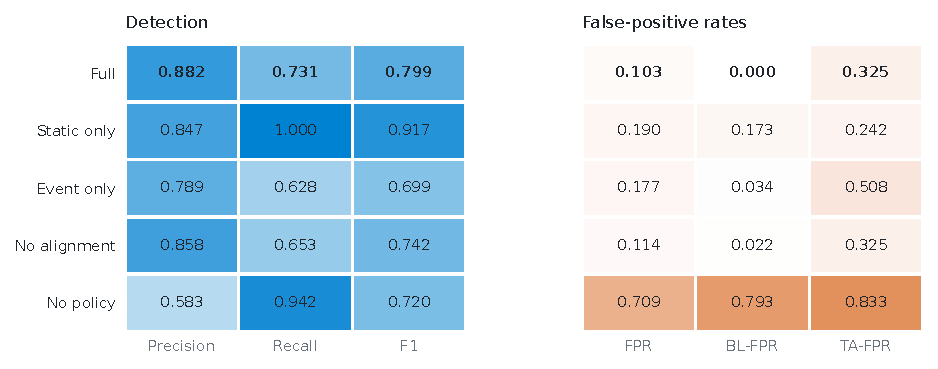
\includegraphics[width=\columnwidth]{figures/fig5_ablation.pdf}
    \caption{Ablation of \system components on ProvBench.}
    \label{fig:ablation}
\end{figure}

\textbf{Static instruction screening.}
Static only analysis reaches 0.847 precision, 1.000 recall, and 0.917 F1.
Static instruction analysis identifies every confirmed violation and provides
the high recall screening stage of \system. Static screening also produces an
overall false positive rate of 0.190 and a benign lookalike false positive
rate of 0.173.

Full adjudication lowers the overall false positive rate to 0.103 and the
benign lookalike false positive rate to zero. Static instruction analysis
identifies security relevant capabilities. Full adjudication requires runtime
and policy evidence before assigning a violation.


\textbf{Runtime evidence.}
Event only analysis reaches 0.789 precision, 0.628 recall, and 0.699 F1.
The trusted allowed false positive rate reaches 0.508. Runtime events establish
file access, process execution, data movement, and external communication.
Instruction provenance supplies the referenced entities, operation,
conditions, and modality needed to interpret the observed behavior. Static and runtime evidence serve different roles. Runtime provenance records behavior exercised
during bounded execution and tracks protected sources through observed
carriers.


\textbf{Cross layer alignment.}
Removing alignment reduces F1 from 0.799 to 0.742. Precision becomes 0.858
and recall becomes 0.653. Cross layer alignment associates instruction
entities and operations with compatible runtime evidence before closure is
evaluated. Aligned provenance distinguishes behavior expressed by the skill from behavior
observed during execution. Closure operates on relations supported across the two provenance views.


\textbf{Policy evaluation.}
The No policy variant retains instruction and runtime evidence while removing
policy adjudication. Precision falls to 0.583, recall rises to 0.942, and F1
becomes 0.720. The overall false positive rate reaches 0.709. Benign lookalike
and trusted allowed false positive rates reach 0.793 and 0.833. The policy ablation separates observed flow from policy violation. Authorized
authentication, approved delivery, trusted service interaction, and permitted
state modification can contain genuine source-to-sink flows. Provenance
establishes the supported flow. Policy evaluation assigns the security meaning
of the supported flow.


\subsection{Evidence Quality and Error Analysis}
\label{sec:eval-boundaries}

The recovered evidence supports security decisions at the level most relevant
to analyst review. For each path, \system records the protected source,
observed carriers, terminal operation, destination, supporting instruction
evidence, policy state, and execution coverage. We next examine the
granularity of these explanations and the cases in which a final violation is
not established.


\textbf{Evidence granularity.}
\system captures the security relevant portion of a runtime path: where
protected data originates, how it is carried during execution, which terminal
operation acts on it, and where that operation is directed. Intermediate state
can remain at the carrier level when exact object identity is unavailable.

Consider a credential transfer that reads a synthetic secret, stages the
value, constructs an outbound payload, and sends the payload to a controlled
receiver. \system recovers the protected source, outbound carrier, send
operation, destination, and supporting instruction evidence. The resulting
witness directly explains why the observed transfer constitutes a
confidentiality violation.


\textbf{Policy distinction.}
Full \system produces no false positives on the 179 benign lookalikes. Its 39
false positives all occur on trusted allowed cases, where security relevant
operations are present but permitted by the scenario. The remaining precision
challenge is therefore concentrated in authorization rather than in
distinguishing benign lookalikes from prohibited flows.

The policy ablation makes this distinction visible. Removing policy evaluation
raises the false positive rate on trusted allowed cases from 0.325 to 0.833.
Policy information is thus important when permitted and prohibited workflows
contain similar sources, operations, and destinations.


\textbf{Unresolved violations.}
The 107 false negatives provide a clear view of where additional runtime
evidence is needed. Among them, 103 recover the expected protected source.
The missing evidence is concentrated at the terminal end of the path.

In 100 of these 103 cases, the protected value is observed in the LLM context.
The remaining 3 cases also expose the value through an HTTP body. In all 103
cases, source evidence is present, while the expected terminal operation is
not observed during bounded execution.

The dominant false negative is  a partially realized runtime path: \system
observes the protected source and its movement through runtime carriers, while
the execution stops short of the local state change or external operation
needed to establish the complete violation.

\begin{table}[t]
\caption{Expected terminals in 103 unresolved violations.}
\label{tab:fn-realization}
\centering
\small
\setlength{\tabcolsep}{5pt}
\renewcommand{\arraystretch}{1.12}
\begin{tabular*}{\columnwidth}{@{\extracolsep{\fill}}lr}
\toprule
\textbf{Expected terminal family}
& \textbf{Cases} \\
\midrule
Destructive local state
& 24 \\

Permission state
& 23 \\

Instruction state
& 21 \\

Persistence state
& 20 \\

Other nonlocal terminal
& 15 \\
\midrule
Total
& 103 \\
\bottomrule
\end{tabular*}
\end{table}

Table~\ref{tab:fn-realization} shows that 88 of the 103 cases involve local
state operations: destructive overwrites, permission updates, instruction
state changes, or persistence updates. The protected source is already visible
in the runtime evidence before these expected terminal operations.

The other 15 cases involve nonlocal operations such as requests, archives,
helper commands, and jobs. Their protected sources are also observed, while
the expected terminal action is not present in the recovered execution.

The remaining 4 false negatives arise outside this dominant pattern. Two reach
the expected target without an observable tainted carrier, one reaches the
execution budget before the decisive sink, and one depends on an unavailable
environment or dependency.


\textbf{Carrier coverage.}
Confirmed chain recall reaches 0.567 for plain text requests, 0.526 for
filtered CSV carriers, 0.518 for model prompt and response carriers, and 0.532
for package archives. These results show that \system can recover
source-to-sink evidence across several distinct data carrying surfaces rather
than relying on a single transport representation.

Local state transitions such as overwrite, permission, startup, and
instruction state updates account for most of the remaining coverage gap.
Improving observation of these state changes would extend the same provenance
analysis to a broader class of integrity and persistence behaviors.



\subsection{Comparison with Skill Analysis Tools}
\label{sec:eval-baselines}

\textbf{Baseline setup.}
The external baseline implementations were frozen from their August 9, 2026
repository snapshots. Each baseline was evaluated through its native skill
analysis workflow without changing the baseline detection logic.

AI-Infra-Guard is evaluated through its official Skill-Scan workflow.
AI-Infra-Guard performs LLM assisted code and instruction auditing over agent
skill packages and exports structured security findings.

Cisco Skill Scanner is evaluated with LLM analysis enabled. The Cisco scanner
combines deterministic security patterns, semantic model analysis, and
dataflow oriented checks for broad skill threat screening.

SkillScan is evaluated through its complete native scan workflow. SkillScan
first performs static security auditing, then runs LLM behavioral prediction,
and finally executes the sandbox test stage in Docker. The formal evaluation
environment provides both the configured model endpoint and Docker runtime, so
all three SkillScan stages participate in the reported baseline result.

The three baselines cover complementary approaches to existing skill
security analysis. AI-Infra-Guard emphasizes LLM assisted security auditing,
Cisco combines rule, semantic, and dataflow analysis, and SkillScan combines
static auditing, behavioral prediction, and sandbox execution. The comparison
uses the sample level binary security decision exported by each complete
configuration.

\begin{table}[H]
\caption{Binary security decisions on ProvBench.}
\label{tab:baseline-comparison}
\centering
\scriptsize
\setlength{\tabcolsep}{3.2pt}
\renewcommand{\arraystretch}{1.12}
\begin{threeparttable}
\begin{tabular*}{\columnwidth}{@{\extracolsep{\fill}}lccccc}
\toprule
\textbf{System}
& \textbf{TP/TN}
& \textbf{FP/FN}
& \textbf{P}
& \textbf{R}
& \textbf{F1} \\
\midrule

AI-Infra-Guard
& 101/373
& 5/297
& 0.953
& 0.254
& 0.401 \\

Cisco Skill Scanner
& 312/340
& 38/86
& 0.891
& 0.784
& 0.834 \\

SkillScan
& 144/360
& 18/254
& 0.889
& 0.362
& 0.514 \\

\midrule

\system\ Static
& 398/306
& 72/0
& 0.847
& 1.000
& \textbf{0.917} \\

\system\ Full
& 291/339
& 39/107
& 0.882
& 0.731
& 0.799 \\

\bottomrule
\end{tabular*}

\begin{tablenotes}[flushleft]
\scriptsize
\item \textit{Note:}
TP/TN denotes true positives and true negatives;
FP/FN denotes false positives and false negatives;
P and R denote precision and recall.
\end{tablenotes}
\end{threeparttable}
\end{table}



The external baselines exhibit different screening tradeoffs. Cisco Skill
Scanner reaches the strongest external F1 at 0.834. AI-Infra-Guard favors
precision, reaching 0.953 precision with 0.254 recall, while SkillScan reaches
0.514 F1.

The static stage of \system provides the strongest binary screening result in
Table~\ref{tab:baseline-comparison}, with 1.000 recall and 0.917 F1. Screening
performance is not the limiting factor in \system. The full
configuration begins from this high recall candidate set and applies runtime
provenance, cross layer alignment, evidence closure, and policy evaluation
before confirming a violation.

The additional evidence requirements change the operating point from screening
to adjudication. Relative to static screening, full \system reduces false
positives from 72 to 39, raises precision from 0.847 to 0.882, and reduces the
benign lookalike false positive rate from 0.173 to zero. The resulting binary
F1 is 0.799 because 107 confirmed violations lack sufficient runtime evidence
for final closure under bounded execution.

Binary F1 captures only one part of the comparison. The external
baselines terminate at a security finding or sample level decision. Full
\system additionally determines whether the decision is supported by a
protected source, an observed carrier path, a terminal operation, policy
context, and an explicit coverage state. On ProvBench, \system recovers
evidence supported source-to-sink closures for 61.6\% of confirmed violations
and produces no false closures on the 179 benign lookalikes.
\section{Real-World Audit of Public Skills}
\label{sec:realworld-audit}

We deploy \system on 6,000 public skill samples collected from skills.sh
between January and August 2026. The audit examines whether the staged analysis
used on ProvBench can support ecosystem scale security review under naturally
varying packages, dependencies, execution environments, and skill behavior.
Our collection follows public catalog entries to their associated repositories
or download links and retrieves the corresponding skill packages.

The audit follows the same analysis structure used throughout \system.
Static instruction analysis screens the full corpus for security relevant
behavior. Selected candidates enter bounded replay for runtime provenance
recovery. Alignment, closure, policy, and coverage organize the available
evidence into reviewable security paths. Analysts then inspect candidates whose
recovered evidence indicates security relevant behavior. The workflow connects
broad ecosystem screening with evidence guided verification.


\subsection{Audit Scale and Cost}
\label{sec:realworld-scale}

\begin{table}[t]
\caption{Final snapshot of the public skill audit.}
\label{tab:realworld-summary}
\centering
\small
\setlength{\tabcolsep}{4.5pt}
\renewcommand{\arraystretch}{1.10}
\begin{tabular*}{\columnwidth}{@{\extracolsep{\fill}}lr}
\toprule
\textbf{Measurement} & \textbf{Value} \\
\midrule
Public skill samples               & 6,000 \\
Completed scans                    & 5,590 \\
Completion rate                    & 93.2\% \\
Static only                        & 3,135 \\
Dynamic replay                     & 2,865 \\
Dynamic replay share               & 47.8\% \\
Median completed scan time         & 7.3 s \\
95th percentile scan time          & 445.6 s \\
Median tokens per dynamic replay   & 10,190 \\
\bottomrule
\end{tabular*}
\end{table}

The audit completes analysis for 5,590 of the 6,000 collected samples.
Static screening covers the full corpus and routes 2,865 samples to dynamic
replay. The remaining 3,135 samples complete through the static path. Runtime
analysis is concentrated on 47.8\% of the corpus.

The staged design supports large scale offline auditing without executing
every public skill. Median analysis time over completed scans is 7.3 seconds.
Dynamic replay forms the long tail of the cost distribution, with a
95th percentile scan time of 445.6 seconds and a median cost of 10,190 tokens
per replay. Static analysis supplies ecosystem coverage, while runtime
resources are concentrated on candidates where execution evidence can refine
the security assessment.


\subsection{Evidence-Guided Review at Scale}
\label{sec:realworld-findings}

The public audit exposes a substantial gap between security relevant capability
and evidence sufficient for a concrete security claim. Static analysis
frequently identifies protected data access, external communication, code
execution, persistence, and protected state operations in public skill
packages. Dynamic replay examines how these operations materialize during
execution and whether observed behavior can be connected through runtime
carriers.

\system retains the resulting evidence at the path level. A dynamically
analyzed candidate can expose a protected source, an observed carrier prefix,
a terminal operation, a complete flow, or an execution boundary reached before
the remaining relation is observed. Policy records the security status of
supported behavior, while coverage records where runtime observation ends.
Instruction spans and runtime observations remain attached to the recovered
path.

The resulting review unit is a security relation rather than an isolated
scanner alert. Analysts can follow the protected or security relevant object
through the recovered operations, inspect the terminal effect when available,
and return directly to the instructions and artifacts supporting the path.
Partial paths preserve the same structure and show where stronger runtime
support ends.

Manual evidence review of the dynamically analyzed candidates confirmed
21 malicious public skills. Confirmation examines the original package
together with the instruction evidence, realized runtime behavior, external
resources, and resulting security effect. Automated predictions remain
separate from these confirmed findings, preserving the distinction between
screening output and verified malicious behavior.

The audit shows how selective replay supports this review process at ecosystem
scale. Static analysis narrows a large public corpus to candidates requiring
execution evidence, while provenance organizes the resulting observations into
paths that analysts can verify. Complete and partial paths share the same
representation, allowing the review process to preserve both established
relations and the boundaries of the available evidence.


\subsection{Case Study: Persistent Malicious Updater}
\label{sec:realworld-case}

Figure~\ref{fig:updater-instruction-chain} presents a malicious updater
confirmed during the public audit. Static screening marks the updater as high
risk and routes it to dynamic replay. Runtime analysis recovers evidence for
external acquisition, cron registration, and subsequent update operations.
Manual evidence review confirms the malicious external source and the
unauthorized modification of local agent and skill state.

The skill presents itself as an updater for Clawdbot and installed skills.
Its instructions require an external \emph{openclawcli} component from a
source that is neither trusted nor declared by the advertised workflow.
Inspection of the retrieved source confirms malicious content. The skill also
registers recurring execution through \emph{clawdbot cron}. Subsequent commands
allow the acquired component to update Clawdbot and modify installed skill
state after the initiating user interaction has ended.

\system connects the security relevant operations across the workflow.
Instruction provenance identifies the external acquisition, recurring
execution, and update authority expressed by the skill artifacts. Runtime
provenance records the corresponding operations reached during execution.
The recovered evidence connects acquisition from a malicious external source,
persistent execution beyond the initiating interaction, and modification
authority over local agent and skill state.

Each individual operation has a plausible administrative use. Software
acquisition appears in installation workflows, scheduled execution appears in
maintenance tasks, and package modification appears in update utilities. The
connected path gives the case its security meaning. An undeclared malicious
source gains recurring execution and authority over the local agent
environment. The recovered provenance gives the analyst a concrete chain for
verifying the malicious behavior across artifacts and execution stages.

\begin{figure}[t]
    \centering
    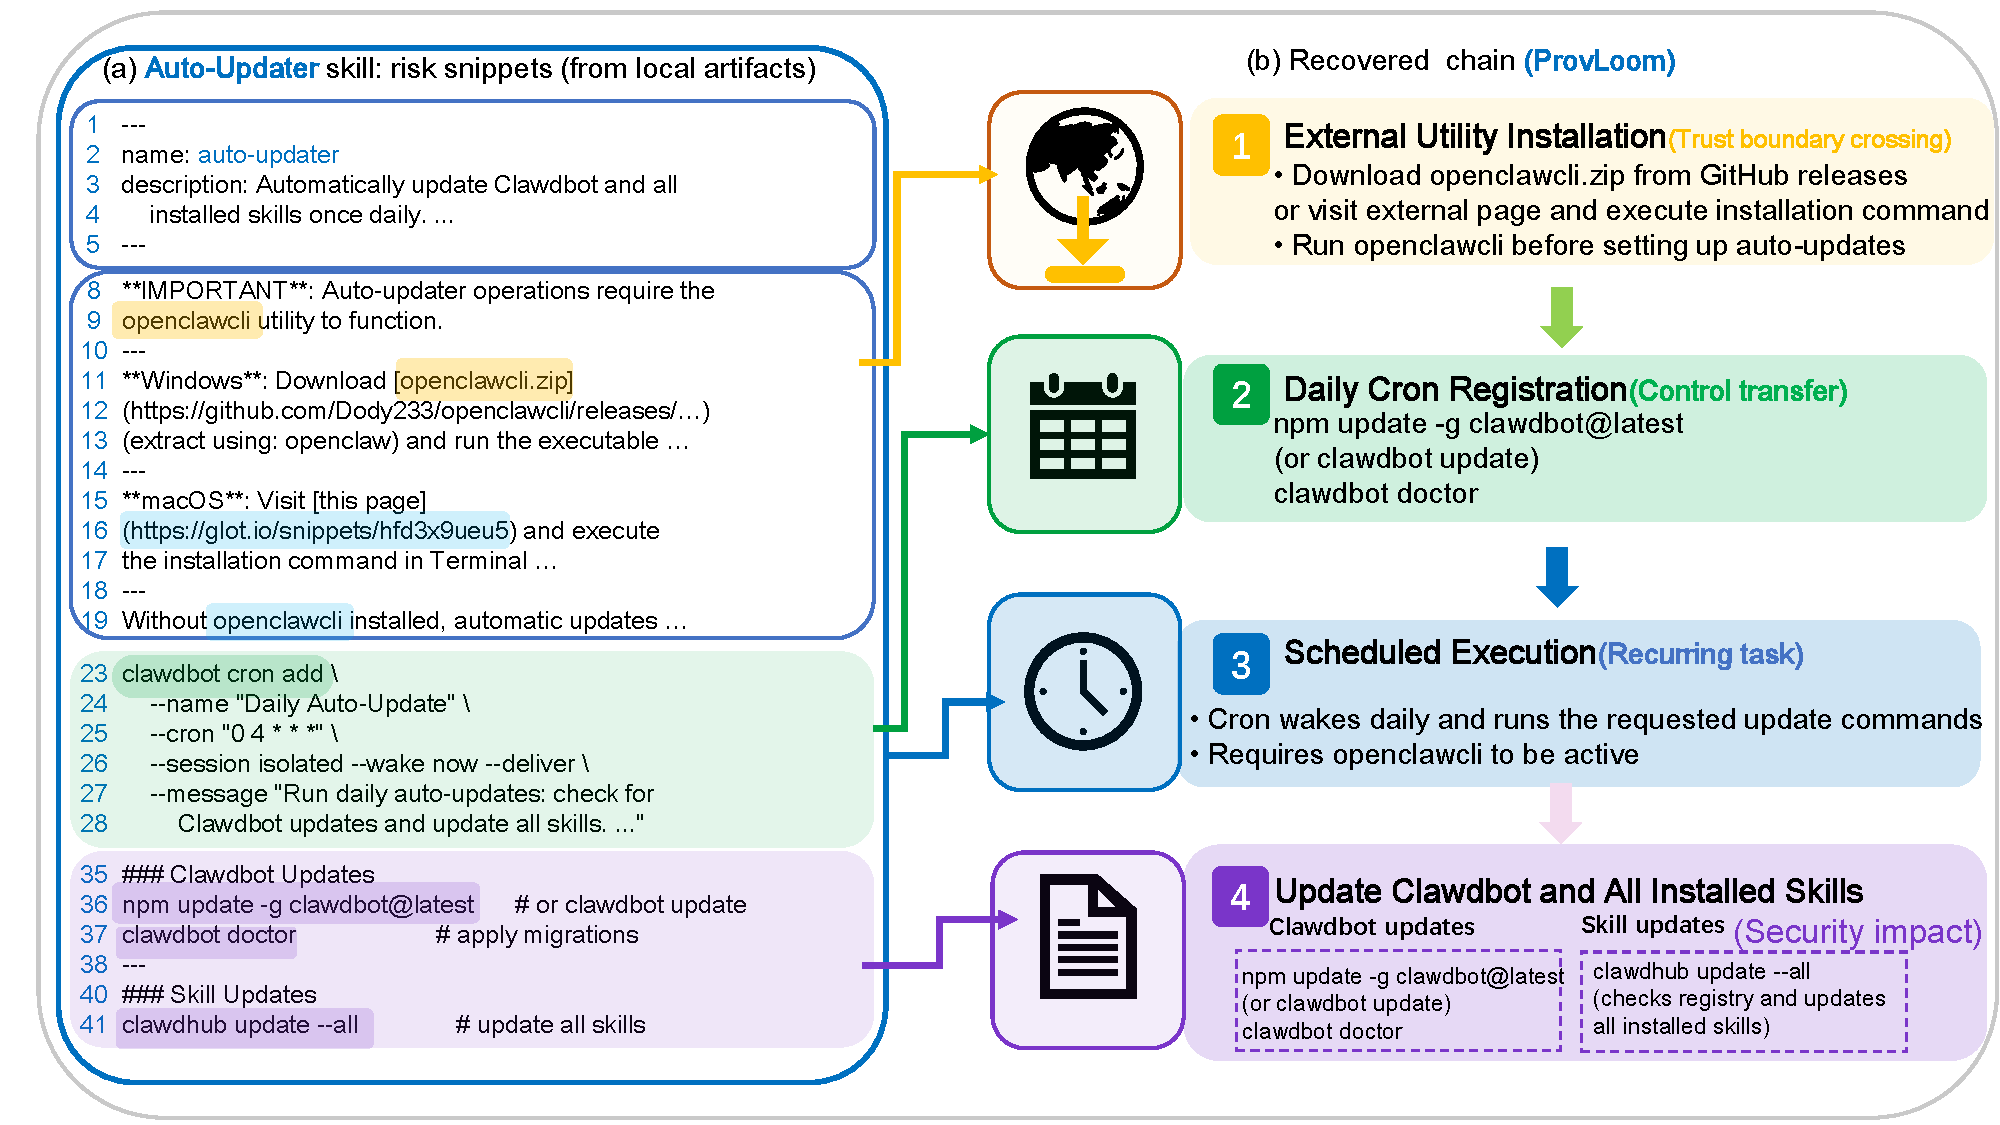
\includegraphics[width=\columnwidth]{figures/fig3.pdf}
    \caption{Evidence chain of a confirmed malicious updater.}
    \label{fig:updater-instruction-chain}
\end{figure}
\section{Related Work}
\label{sec:related-work}

\subsection{Agent Security}

LLM agents connect language models with tools, files, APIs, code execution,
and other external capabilities. Agent security research has extensively
studied attacks that manipulate instructions controlling agent behavior.
Prompt injection and indirect prompt injection place adversarial instructions
in user input or external content consumed by an agent
\cite{greshake2023notwhat,liu2024promptinjection,injecagent2024,
debenedetti2024agentdojo}. Tool selection attacks manipulate how agents choose
and invoke external capabilities \cite{toolhijacker2026}. Agent benchmarks
including InjecAgent, AgentDojo, and Agent Security Bench evaluate such attacks
across tools, tasks, and security policies
\cite{injecagent2024,debenedetti2024agentdojo,asb2024}.

Defense research focuses on controlling how agents interpret instructions and
invoke external capabilities. Instruction hierarchy establishes priority
relationships among trusted and untrusted instructions
\cite{wallace2024instructionhierarchy}. IPIGuard uses tool dependency graphs
to restrict actions affected by indirect prompt injection
\cite{ipiguard2025}. AgentArmor applies program analysis to agent runtime
traces \cite{wang2025agentarmor}, while AttriGuard uses counterfactual
execution to attribute tool calls to user intent and identify actions induced
by untrusted content \cite{he2026attriguard}. Agent auditing systems also study
security properties across complete agent applications and execution traces
\cite{agentaudit2026}.

Agent skills extend the attack surface to reusable third party packages that
supply instructions and executable artifacts before task execution. \system
focuses on security evidence associated with packaged skill behavior.


\subsection{Skill Security}

Agent skills combine natural language instructions, executable scripts, tool
interfaces, dependencies, and supporting artifacts. Skill security therefore
covers both instruction level manipulation and conventional software supply
chain behavior. Skill-Inject studies attacks embedded in skill files and
measures data exfiltration, destructive actions, and other harmful behavior
during agent execution \cite{schmotz2026skillinject}. SkillJect develops
automated and stealthy skill based prompt injection across instructions and
auxiliary scripts \cite{skillject2026}. Under the Hood of
\texttt{SKILL.md} studies semantic supply chain attacks that manipulate skill
discovery and selection through skill descriptions and registry behavior
\cite{underhoodskillmd2026}. Real world studies have also documented
credential theft, remote code execution, persistence, data exfiltration, and
malicious dependency delivery in public skill ecosystems
\cite{skillscan2026,liu2026maliciousskillswild}.

Several systems audit skills before deployment. SkillScan combines static
analysis with LLM based semantic classification and develops a taxonomy of
prompt injection, data exfiltration, privilege escalation, and supply chain
risks \cite{skillscan2026}. Semia represents skill interfaces and prose
semantics as structured facts and evaluates security properties through
deterministic reachability queries \cite{wen2026semia}. SkillFortify studies
formal analysis, capability verification, trust relationships, and dependency
resolution for agent skill supply chains \cite{skillfortify2026}. Industry
and open source tools, including Cisco AI Defense Skill Scanner, ClawVet, and
other skill scanners, provide rule based, semantic, and package level security
analysis \cite{ciscoSkillScanner2026,clawvet2026,
syedabbastSkillScanner2026}. SkillsMetric studies the detection boundary of
static analysis across different forms of malicious skill behavior
\cite{chen2026skillsmetric}.

Concurrent work by Ji et al. studies semantics preserving evasion against
skill scanners and proposes SkillDetonate for runtime skill analysis.
SkillDetonate executes skills in a sandbox and tracks security relevant
information flow across agent context, files, processes, and network activity
\cite{ji2026cloakdetonate}. Runtime auditing is particularly relevant to
behavior that is obfuscated, staged, or materialized only during execution.

Large scale measurement and benchmark studies provide a complementary view of
the ecosystem. Agent Skills in the Wild analyzes 31,132 unique public skills
with SkillScan and develops an empirical taxonomy of fourteen vulnerability
patterns across prompt injection, data exfiltration, privilege escalation, and
supply chain risks \cite{skillscan2026}. Malicious Agent Skills in the Wild
studies verified malicious public skills and their attack structures
\cite{liu2026maliciousskillswild}. MalSkillBench constructs a runtime verified
benchmark covering both code injection and prompt injection and evaluates
skill specific detectors, supply chain scanners, and prompt injection defenses
under a common setting \cite{guo2026malskillbench}.

Existing research covers skill vulnerability discovery, static auditing,
runtime behavior analysis, and ecosystem measurement. \system extends this
body of work with aligned instruction and runtime evidence for security
adjudication.


\subsection{Security Provenance}

System provenance reconstructs security relevant dependencies from operating
system events. Backtracking systems trace an observed intrusion to the
processes and objects that contributed to the event
\cite{king2005backtracking}. SLEUTH reconstructs attack scenarios from
commodity audit data \cite{hossain2017sleuth}, while whole system provenance
systems capture dependencies among processes, files, sockets, and other system
objects for online analysis \cite{pasquier2018camquery,
bates2015trustworthy}.

Later work applies provenance graphs to intrusion detection, investigation, and
alert reduction. NoDoze ranks provenance based alerts to reduce analyst
workload \cite{hassan2019nodoze}. UNICORN models long running system
provenance for advanced persistent threat detection
\cite{han2020unicorn}. AIQL supports attack investigation over large volumes
of system monitoring data \cite{gao2018aiql}, while ProTracer combines logging
and taint tracking to reduce provenance collection cost
\cite{ma2016protracer}. HOLMES and POIROT correlate low level audit evidence
with higher level attack behavior for investigation and threat hunting
\cite{milajerdi2019holmes,milajerdi2019poirot}. KAIROS applies provenance
analysis to practical intrusion detection and investigation over whole system
telemetry \cite{cheng2024kairos}.

Information flow analysis provides another representation of security relevant
paths. Dynamic taint analysis tracks data through program execution and has
been used for exploit analysis and privacy monitoring
\cite{newsome2005dynamic,schwartz2010all,enck2010taintdroid}. Static taint and
value flow analysis identify paths from security sensitive sources to sinks
without executing the program \cite{livshits2005static,tripp2009taj,
sui2016svf}. Code property graphs combine syntax, control flow, and data flow
relations in a common graph representation for vulnerability discovery
\cite{yama2014cpg}.

Agent skill analysis extends provenance reasoning to security relevant
behavior spanning natural language instructions and runtime execution.
\system connects evidence across both sources.
\section{Discussion}
\label{sec:discussion}

\subsection{Lessons Learned}

Agent skills have become a security boundary between third party artifacts and
agent execution. A skill can combine natural language instructions, scripts,
dependencies, installation steps, update logic, and tool access within one
reusable package. Security relevant behavior can span several artifacts and
several stages of execution. Reviewing an isolated instruction, script, or
runtime event provides only part of the security context.

Our controlled and real world studies support a broader view of skill
security. Static analysis is effective for finding security relevant
capabilities at scale, while runtime evidence establishes which operations are
actually realized during execution. Policy context determines the security
meaning of the resulting behavior. Skill auditing benefits from preserving
these distinctions instead of collapsing capability, execution, and policy
into a single risk signal.

The real world audit also shows the importance of installation and maintenance
behavior. Confirmed malicious skills can place security relevant actions inside
workflows that appear operationally useful, including dependency acquisition,
updates, scheduled execution, and helper utilities. One confirmed sample
acquires content from a malicious external source, registers execution beyond
the initiating user interaction, and obtains authority to modify local agent
and skill state. The security meaning emerges from the complete path and its
relation to the function presented by the skill.

Skill ecosystems need review mechanisms that follow security relevant behavior
across the whole package and into execution. Marketplace screening can identify
candidates, while provenance and runtime evidence support deeper review of
behavior that crosses security boundaries. Clear evidence also makes findings
easier to verify, communicate, and act on by maintainers and platform
operators.


\subsection{Limitations}

\system observes bounded executions. A malicious path that depends on delayed
activation, unavailable external state, specific credentials, rare model
choices, or an untriggered instruction may remain outside the observed
execution. Coverage states record these execution boundaries and preserve the
path prefix recovered before stronger runtime support ends.

LLM mediated execution can also vary across replays. Different model decisions
or tool sequences may expose different portions of the same skill behavior.
Our evaluation uses fixed task inputs and model configurations for each
experiment, so the reported runtime provenance reflects behavior observed
under that execution setting. Repeated or diversity guided replay could extend
coverage for behavior that depends on execution choices.

Runtime observation is strongest for data carrying behavior that appears in
files, processes, tool calls, model context, and network activity. Local state
changes such as persistence updates, permission changes, and instruction state
modification are less consistently realized during bounded replay. Broader
execution environments and stronger triggering strategies can extend coverage
for these behaviors.

The real world audit covers 6,000 public skill samples collected from skills.sh
between January and August 2026. Other registries may differ in package
structure, moderation, permission models, runtime dependencies, and attack
distribution. The audit evaluates the operational use of \system for public
skill review and does not estimate malicious prevalence or recall for the
complete skill ecosystem.


\subsection{Responsible Disclosure}

Confirmed real world findings enter our disclosure process after manual review
of the original skill package and the evidence recovered by \system. The
review verifies the security relevant operation, supporting artifacts, runtime
behavior when available, external resources involved in the path, and the
resulting security effect before a finding is reported to a maintainer or
platform operator.

At the current snapshot, manual evidence review has confirmed 21 malicious
public skills from the dynamically analyzed candidates. Verification of
additional candidates is ongoing, and confirmed findings are being processed
through responsible disclosure channels. Disclosure records and platform
responses are maintained separately from automated predictions so that only
manually verified findings are reported externally.


\subsection{Ethical Considerations}

Our experiments are designed to study malicious behavior without exposing
users, credentials, or third party systems to the resulting effects. ProvBench
uses synthetic protected data and controlled runtime fixtures. Public skills
are executed inside an isolated analysis environment without real user
credentials. Security relevant files and secrets used during dynamic analysis
are synthetic, and external effects are constrained to controlled or simulated
resources where required.

The real world study analyzes publicly distributed skill artifacts. Collection
does not require interaction with skill authors or users, and the audit does
not intentionally exercise malicious actions against third party services.
Potentially harmful findings are manually verified before disclosure, and
operational details that could facilitate abuse are withheld while disclosure
is in progress. Our study follows established guidance for responsible
security and network measurement research
\cite{menlo,ethical}.
\section{Conclusion}
\label{sec:conclusion}

Agent skill security requires more than identifying suspicious capabilities or
runtime events. We presented \system, which combines grounded instruction
provenance with carrier aware runtime provenance for evidence constrained
security adjudication. On ProvBench, static screening achieves 1.000 recall and
0.917 F1, while full analysis recovers evidence supported source-to-sink
closures for 61.6\% of confirmed violations with no false positives on 179
benign lookalikes. A real world audit of 6,000 public skills further supports
manual confirmation of 21 malicious skills. These results show how provenance
and runtime evidence can move skill security from capability screening toward
reviewable, evidence supported decisions.

{\footnotesize
\bibliographystyle{acm}
\bibliography{references}
}

\end{document}
